% ------------------------------------------------------------------------ %
% !TEX encoding = UTF-8 Unicode
% !TEX TS-program = pdflatex
% !TEX root = ../Tesi.tex
% !TEX spellcheck = it-IT
% ------------------------------------------------------------------------ %
%
% ------------------------------------------------------------------------ %
% 	STATO DELL'ARTE
% ------------------------------------------------------------------------ %
%
\chapter{State of the Art}
%
\label{cap:statoarte}
%
% ------------------------------------------------------------------------ %
%
\section{Android OS} \label{androidos}
\par As already mentioned in \ref{motivation}, the Android operating system is an open source OS developed by Google based on Linux kernel, that can be installed on many different kind of devices.\\
In this section i want to give to the reader the basic knowledge of the Android framework to understand why and how the operating system works.
\subsection{Brief History} \label{briefhist}
\par
The Android era officially began on October 22nd, 2008, when the \textit{T-Mobile G1} launched in the United States \cite{verge2011android}.\\
At that moment the company of mountain view, Google, felt the need to create a new operating system which was able to be installed on most modern mobile phones of the time. To meet this need the Google engineers created an OS that was based on the Linux kernel, lightweight enough and ease to be used with simple hand gestures by touching the screen of the phone.\\

\begin{figure}[h]
	\centering
	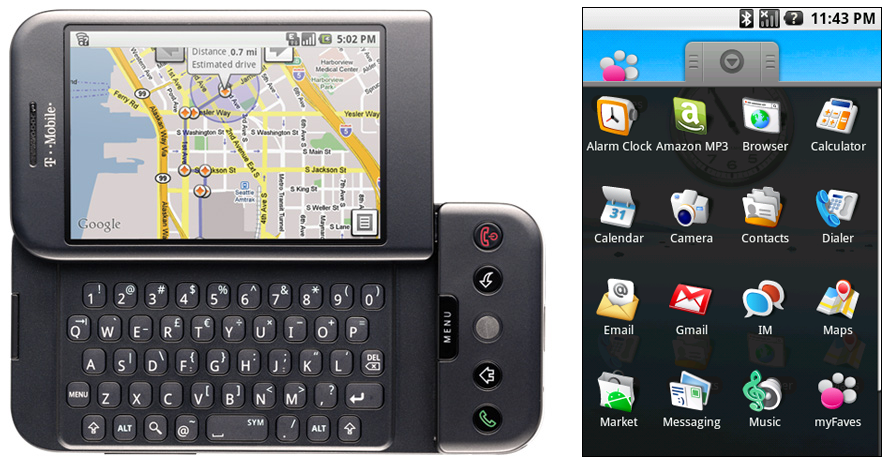
\includegraphics[width=0.8\textwidth]{T-MobileG1Android1menu}
	\caption{The T-Mobile G1 and the Android 1.0 menù}
	\label{2.1:The T-Mobile G1 and the Android 1.0 menù}
\end{figure}

The main characteristic of the OS were and are also now:
\begin{itemize}
	\item The pull-down notification window.
	\item Home screen widgets.
	\item The Android Market.
	\item Google services integration (eg. Gmail).
	\item Wireless connection technologies (eg Wi-Fi and Bluetooth)
\end{itemize}
The success of the first version of the brand new mobile operating system and the open source philosophy guaranteed the fast spread of the Android devices all over the world. In few years Google improved and released many version of the OS and with the help of the market growth Android has become a complete os. 
In the table below there is a brief description of the various distribution of the Android OS at the time of writing of this document.\\
\begin{table}[h]
	%
	\caption{Android versions}
	%
	\label{tab:vers}
	%
	\centering
	%
	\begin{tabular}{llll}
		%
		\toprule
		%
		\textbf{Name} & \textbf{Version}  & \textbf{Release Date} & \textbf{API Level}\\
		%
		\midrule
		%
		Alpha &	1.0 & September 23, 2008 & 1 \\
		Beta & 1.1 & February 9, 2009 & 2 \\
		Cupcake & 1.5 & April 27, 2009 & 3 \\
		Donut &	1.6 & September 15, 2009 & 4 \\
		Eclair & 2.0 – 2.1 & October 26, 2009 & 5–7 \\
		Froyo & 2.2 – 2.2.3 & May 20, 2010 & 8 \\
		Gingerbread & 2.3 – 2.3.7 & December 6, 2010 & 9–10 \\	
		Honeycomb & 3.0 – 3.2.6 & February 22, 2011 & 11–13 \\
		Ice Cream Sandwich & 4.0 – 4.0.4 & October 18, 2011 & 14–15 \\
		Jelly Bean & 4.1 – 4.3.1 & July 9, 2012 & 16–18 \\
		KitKat & 4.4 – 4.4.4 & October 31, 2013 & 19 \\
		Lollipop & 5.0 – 5.1.1 & November 12, 2014 & 21–22 \\
		Marshmallow & 6.0 – 6.0.1 & October 5, 2015 & 23 \\
		Nougat & 7.0 – 7.1.1 & August 22, 2016 & 24–25 \\
		%
		\bottomrule
		%
	\end{tabular}
	%
\end{table}
 As we can see in \tablename~\ref{tab:vers} there are, currently, 25 level of the Android \textit{API} (Application programming interface
 ) which developers can use to build Android applications. In particular various API levels introduce innovations in the OS but, applications developed using an higher \textit{API level} can not be executed in a device running lower versions of the operating system. This is a second major limitations for the \textit{"Android ecosystem"}, moreover as mentioned before, the Android OS is released under an open source license, which is great for the developer, but which prevents Google to provide updates, in a centralized way, to all devices. For this reason there are currently many active devices running different versions of the mobile OS, as we can check in \tablename~\ref{tab:chart}, which shows, in percentage, the fragmentations of active machines running Android OS.\\
 \begin{table}[h]
 	%
 	\caption{Android OS versions fragmentation}
 	%
 	\label{tab:chart}
 	%
 	
 	%
 	\begin{minipage}{0.5\textwidth}
 		\centering
 		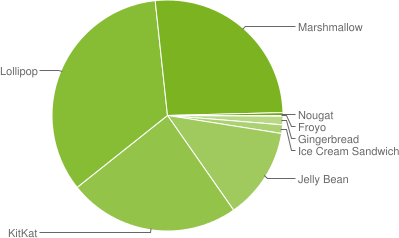
\includegraphics[width=0.9\textwidth]{androidversionchart}
 		 \captionof{figure}{Android OS fragmentation chart}
 		\label{2.2:Android fragmentation chart}
 		
 	\end{minipage}
 ~\hfill~
 \begin{minipage}{0.5 \textwidth}
 	\centering
 	\begin{tabular}{lll}
 		%
 		\toprule
 		%
 		\textbf{Version}  & \textbf{API Level} & \textbf{Distribution}\\
 		%
 		\midrule
 		%
 		2.2 & 8 & 0.1\% \\
 		2.3.3 - 2.3.7 & 10 & 1.2\% \\
 		4.0.3 - 4.0.4 & 15 & 1.2\% \\
 		4.1.x & 16 & 4.5\% \\
 		4.2.x & 17 & 6.4\% \\
 		4.3 & 18 & 1.9\% \\
 		4.4 & 19 & 24.0\% \\
 		5.0 & 21 & 10.8\% \\
 		5.1 & 22 & 23.2\% \\
 		6.0 & 23 & 26.3\% \\
 		7.0 & 24 & 0.4\% \\
 		%
 		\bottomrule
 		%
 	\end{tabular}
\end{minipage}
 	%
 \end{table}
Data in \tablename~\ref{tab:chart} were collected during a 7-day period ending on December 5, 2016, by Google. Any versions with less than 0.1\% distribution are not shown \cite{devandroiddash}.
\subsection{Structure}
\par
Android is an operating system based on the Linux kernel. The project responsible for developing the Android system is called the \textit{Android Open Source Project (AOSP)} and it lead by Google.
\begin{figure}[h]
	\centering
	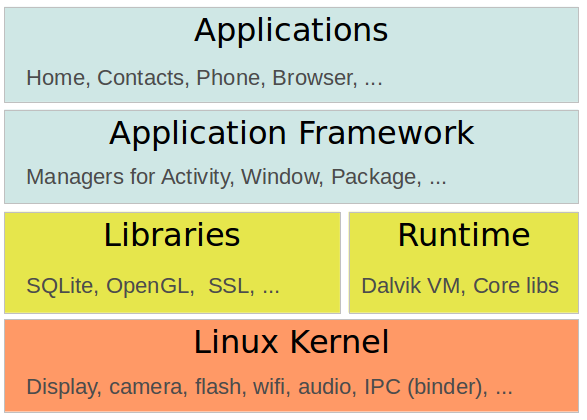
\includegraphics[width=0.8\textwidth]{oslevels}
	\caption{Android OS 4 layers}
	\label{fig:2.3}
\end{figure}

The OS can be divided into the four layers as depicted the \figurename~\ref{fig:2.3}. An Android application developer typically works with the two layers on top to create new Android applications \cite{vogel2016android}.

\paragraph{Linux Kernel} is the most flexible operating system that has ever been created. It can be tuned for a wide range of different systems, running on everything from a radio-controlled model helicopter, to a cell phone, to the majority of the largest supercomputers in the world \cite{hartman2006linux}. This is in practice the communication layer for the underlying hardware.
\paragraph{Runtime and Libraries} \par Runtime is the term used in computer science to designate the software that provides the services necessary for the execution of a program.There are two different \textit{"runtime systems"} which can work with the Android OS:
\begin{itemize}
	\item \textit{Dalvik VM} is an optimized version for low memory devices of the \textit{Java Virtual Machine (JVM)} used in Android 4.4 and earlier version. It is stack based and it works by converting using a \textit{just-in-time (JIT)}, each time an application is executed, Android's \textit{bytecode} into machine code.
	\item \textit{ART (Android Runtime)} introduced with Android 4.4 KitKat. This runtime uses an \textit{AOT (Ahead-of-Time)} approach, with which code is compiled during the installation of an application and then is ready to be executed.
\end{itemize}
\par Standard Android libraries are for many common framework functions, like, graphic rendering, data storage, web browsing. \cite{vogel2016android}. This layer contains also standard \textit{java libraries}.
\paragraph{Application Framework}\label{appframework} is the layer that contains the Android components for the application such as activities, fragments, services and so on. 
\paragraph{Applications} are pieces of software written in \textit{java code} running on top the other layers.

\subsection{Application Framework}
In this section I want to give some details of the application composition and work flow to better understand the subsequent sections in which I will describe the given problem and the proposed solution.\\
As briefly described in \ref{appframework} the Android application framework \textit{("AppFramework")} is the core of the Android \textit{development API}. It contains useful and needed components to build native apps.\\
The main components with which each application is composed are:

\paragraph{Intents} are objects that initiate actions from other app components, either within the same program \textit{(explicit intents)} or through another piece of software on the device \textit{(implicit intents)}.
Acconrding to the official Google's Android for developer documentation, an Intent is a sort of messaging object which can be used to request an action from another application component (eg. activities). There are three fundamental use cases:
\begin{itemize}
	\item Starting an activity: we will see that activities represents a single screen in Android applications, intents allow to start activities by describing them and carrying any necessary data.
	\item Starting a service: I will explain later in deeper details that services are component which performs operations in background. As for the activities, services are initialized through intent and in the same way they describe the service to start and carries any necessary data.
	\item Delivering a broadcast: broadcast is a message that any app can receive. The system delivers various broadcasts for system events, such as when the system boots up or the device starts charging.
\end{itemize}

As already mentioned there are mainly two categories of intents:
\begin{itemize}
	\item explicit intents, used when it is needed to start component within the same application. As the name implies explicit intents call components by using by name (the full \textit{class object} name), for example, it is possible to start a new activity in response to a user action or start a service to download a file in the background.
	\item implicit intents do not name a specific component, but instead declare a general action to perform, which allows a component from another app to handle it. For example, if you want to show the user a location on a map, you can use an implicit intent to request that another capable app show a specified location on a map \cite{devandroidintent}.
\end{itemize}

\begin{figure}[h]
	\centering
	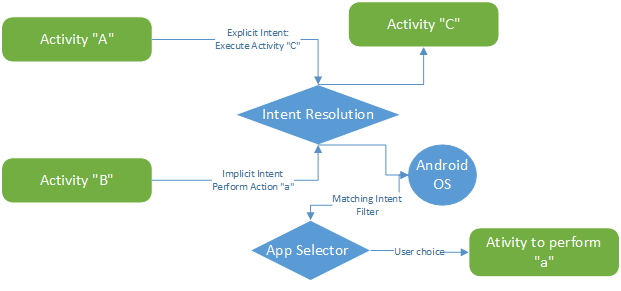
\includegraphics[width=0.9\textwidth]{intentresolution}
	\caption{Intent resolution mechanism}
	\label{fig:2.4}
\end{figure}

The \figurename~\ref{fig:2.4} explains well how an intent is resolved by the OS whether it is implicit or explicit. When an implicit intent needs to be resolved, the OS searches applications which can handle it by means of \textit{intent filters}.A Intent filter specifies the types of intents that an activity, service, or broadcast receiver can respond to. The Android System searches all apps for an intent filter that matches the intent to be resolved. When a match is found, the system starts the matching component, or, if there are more than one, let the user select the preferred action to be performed.

\paragraph{Activities} are one of the fundamental building blocks of apps on the Android platform. They serve as the entry point for a user's interaction with an app, and are also central to how a user navigates within an app. \cite{devandroidactivity}. An activity is the entry point for interacting with the user. It represents a single screen with a user interface \textit{GUI}: in this way activities are containers for other Android's GUI elements (eg. buttons, textviews,...).

\paragraph{Services} is a general-purpose entry point for keeping an app running in the background for all kinds of reasons. It is a component that runs in the background to perform long-running operations or to perform work for remote processes. A service does not provide a user interface \cite{devandroifundamentals}. 

\paragraph{Broadcast Receivers} are components that enable the system to deliver events to the app outside of a regular user flow, allowing the app to respond to system-wide broadcast announcements. Because broadcast receivers are another well-defined entry into the app, the system can deliver broadcasts even to applications that aren't currently running \cite{devandroifundamentals}.

\subsection{Security}\label{androidsecurity}
\par
As described in \ref{briefhist} Android was born to be a good mobile OS and it is mainly for this reason that the system is designed to protect personal and sensible data form malicious guys.\\
Like the rest of the system, Android's security model also takes advantages of the security features offered by the Linux kernel. Linux is a \textit{multiuser OS} and its kernel can isolate user data from one another: one user can not access another user's file unless explicitly granted permission. Android takes advantages of this user isolation, considering each application a different user provided with a dedicated \textit{UID (User ID)} \cite{elenkov2014android} Android in fact, is designed for smartphones that are personal devices and do not need, usually, a multi physical user support.
The most important security techniques adopted by Android are:

	\paragraph{Application Sandboxing} Android automatically assigns a unique \textit{AppID} (Linux UID) when an application is installed and then executed that specific app in a dedicated process as that UID. This technique isolate all the applications at process level and additionally each app has permissions to read/write a specific and dedicated directory.
	
	\paragraph{Permissions} Since application are sandboxed and do not have the rights to read/write date outside them, it is possible to grant additional rights to android applications by explicitly asking them. Those access rights are called \textit{permission}. Applications can request permissions by listing them in a configuration file called \textit{android manifest}. In Android 5.1 and earlier versions permission are inspected and granted at installation time, when the user is alerted with a dialog box in which are listed permissions the application to be installed needs to work properly and when granted cannot be revoked. Starting from android 6.0 permission are asked the first time that an application need them, and when are granted they can be revoked manually in the OS settings for that specific application.
	
		\begin{figure}[h]
		\centering
		\begin{minipage}[c]{.45\textwidth}
			\centering\setlength{\captionmargin}{0pt}%
			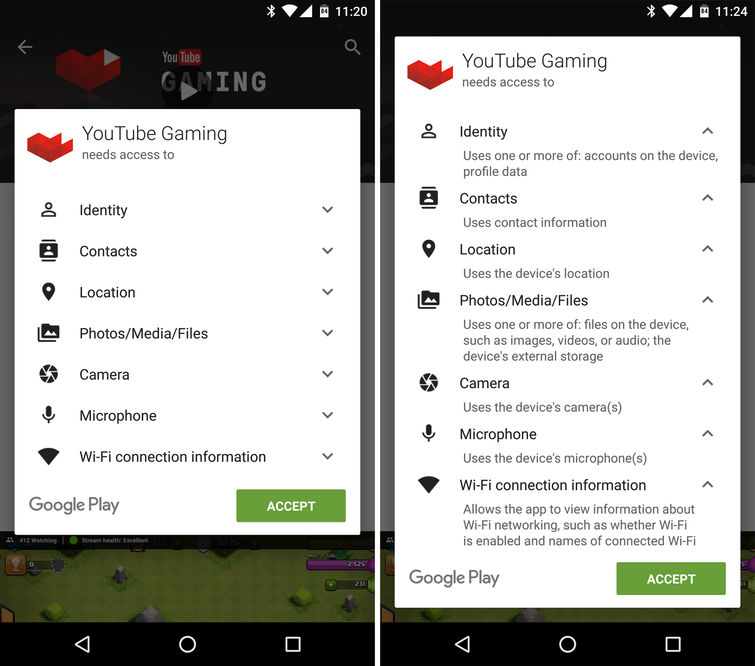
\includegraphics[width=.9\textwidth]{51permissions}
			\caption{Android 5.1- permission example}
		\end{minipage}%
		\hspace{10mm}%
		\begin{minipage}[c]{.45\textwidth}
			\centering\setlength{\captionmargin}{0pt}%
			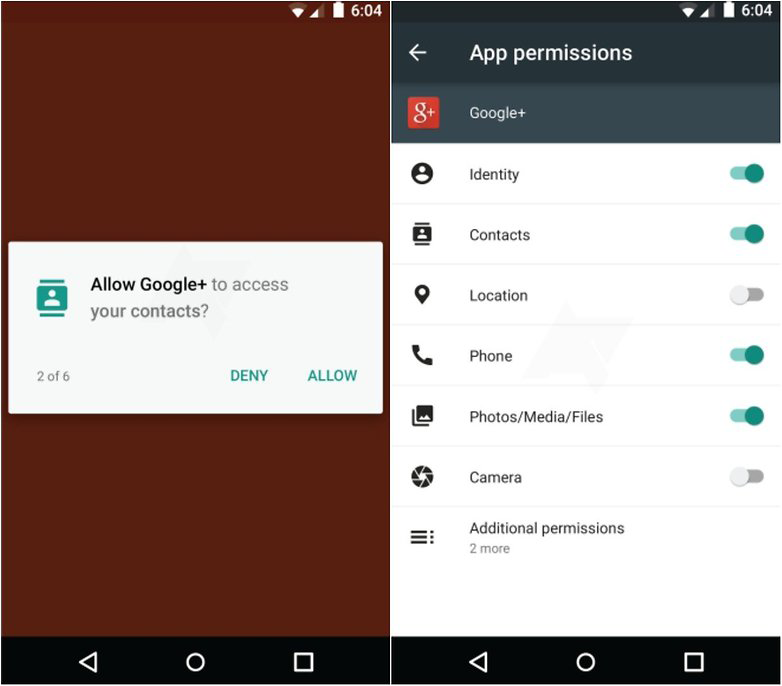
\includegraphics[width=.9\textwidth]{60permissions}
			\caption{Android 6.0+ permission example}
		\end{minipage}
		\caption{Android permission Examples\label{fig:Andorid permission Examples}}
	\end{figure}

	\paragraph{SeLinux} Security Enhanced Linux, is a \textit{mandatory access control (MAC)} system for the Linux operating system. With a MAC the operating system constrains the ability of a subject or initiator to access or generally perform some sort of operation on an object or target. Starting in Android 4.3, SELinux provides a mandatory access control (MAC) umbrella over traditional discretionary \textit{access control (DAC)} environments. For instance, software must typically run as the root user account to write to raw block devices. In a traditional DAC-based Linux environment, if the root user becomes compromised that user can write to every raw block device. However, SELinux can be used to label these devices so the process assigned the root privilege can write to only those specified in the associated policy.
 	In this way, the process cannot overwrite data and system settings outside of the specific raw block device \cite{secure2017android}.

\subsection{Connectivity}\label{connectivity}
\par
As already amply explained previously many Android design choices are due to the fact that it was thought for mobile devices which must have connectivity to intercommunicate among them.\\
With the evolution of various wireless communication technologies, Android devices, nowadays, are equipped whit different kinds of modulus, the most common are:
\begin{itemize}
	\item Wi-Fi
	\item Bluetooth
	\item NFC
	\item Cellular Network
\end{itemize}
The Android Os provide a full library to operate with these technologies and it is possible to integrate in applications the possibility to communicate over these wireless modules.
With the \textit{Android connectivity API} data can be send and received in an efficient way.\\\\
\par
I have only quickly listed some features and possible issues of my source, to have a complete idea it is possible to read all the official Android documentation in \cite{devandroifundamentals}.
 
\section{Distributed System} \label{distsys}
In this section I want to give to the reader some basics about distributed systems, including technical details and examples to make the proposed solution easier to understand.
\subsection{Definition}\label{distdef}
\textit{A distributed system is a collection of independent computers that appears to its users as a single coherent system.}\\
This definition has several important aspects. The first one is that a distributed system consists of components (i.e., computers) that are autonomous. A second aspect is that users (be they people or programs) think they are dealing with a single
system. This means that one way or the other the autonomous components need to collaborate \cite{tanenbaum2010distributed}.\\
\begin{figure}[h]
	\centering
	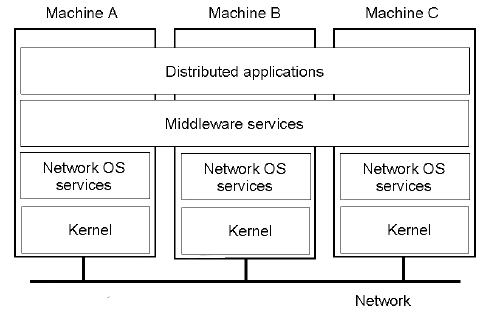
\includegraphics[width=0.8\textwidth]{distributedsystem}
	\caption{Distributed system structure}
	\label{fig:2.8}
\end{figure}
In \figurename~\ref{fig:2.8} it is possible to see how can be structured a distributed system: a the top we have the real distributed application, which is the final interface to be used, under which it is possible to have different combinations of services used to make communicate different machines that may use different operating systems. The real magic is done by the layer called \textit{middleware service} in the picture. A middleware in computer science is a set of software which act as intermediaries between structures and computer programs, allowing them to communicate in spite of the diversity of protocols or running OSs.

\subsection{Challenges} \label{chall}
There are many challenges in distributed systems field: distributed applications are often really complex and easily exposed to physical and technical failures because of their nature. Major challenges and property to be considered when developing a system of this kind are:

\begin{figure}[h]
	\centering
	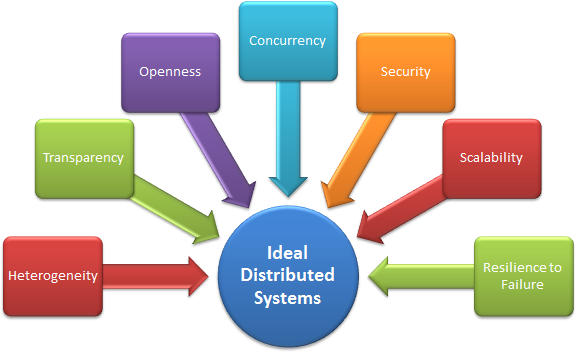
\includegraphics[width=0.8\textwidth]{challengesdistributedsystems}
	\caption{Distributed system challenges}
	\label{fig:2.9}
\end{figure} 

\begin{itemize}
	\item Heterogeneity, is a major challenge because there are many different component to be considered, distributed systems may be developed for example for different hardware, networks, operating systems and programming languages.
	\item Openness, determines whether a system can be extended and reimplemented in various ways, so distributed systems should use standards as much as possible. Developers should always choose the simplest ways during design and implementation phases.
	\item Security, is crucial in many areas of computer science and specially in distributed systems, where data are exchanged by a several number of machines.
	\item Scalability, is the ability to easily increase the size of the system in terms of users/resources and geographic
	span.
	\item Failure handling, is important because having different components working together to a common goal means that distributed system can fail in many ways. This raises some issue: it would be nice id distributed systems can detect, mask and tolerate failures.
	\item Concurrency in distributed systems is a matter of
	fact, access to shared resources (information or services)
	must be carefully synchronized.
	\item Transparency level are listed in \tablename~\ref{tab:transparency}
	\begin{table}[h]
		%
		\caption{Transparency levels}
		%
		\label{tab:transparency}
		%
		\centering
		%
		\begin{tabular}{ll}
			%
			\toprule
			%
			\textbf{Transparency} & \textbf{Description}\\
			%
			\midrule
	%
			Access & Hide differences in data representation and how a resource is accessed\\
			Location & Hide where a resource is located\\
			Migration & Hide that a resource may move to another location\\
			Relocation & Hide that a resource may be moved to another location while in use\\
			Replication & Hide that a resource may be shared by several competitive users\\
			Concurrency & Hide that a resource may be shared by several competitive users\\
			Failure & Hide the failure and recovery of a resource\\
			Persistence & Hide whether a (software) resource is in memory or on disk\\
			%
			\bottomrule
			%
		\end{tabular}
		%
	\end{table}
\end{itemize}

\subsection{Comunication Model}
\paragraph{Remote procedure call (RPC)}
\paragraph{Remote method invocation (RMI)}
\paragraph{Message oriented}

\subsection{Architectures}
\par
There are actually many different kinds of distributed systems which can be classified in by means of their architecture composition.
\paragraph{Client-Server} is the most common architecture in computer systems, there are many variants depending on the internal division of its components but it has a common separation of duties. Server side components are passive and wait for clients invocations.Client computers provide an interface to allow a computer user to request services of the server and to display the results it returns. Servers wait for requests to arrive from clients and then respond to them. Ideally, a server provides a standardized transparent interface to clients so that clients need not be aware of the specifics of the system (i.e., the hardware and software) that is providing the service. The communication adopted by these kind of systems is message oriented or through RPC.
\begin{figure}[h]
	\centering
	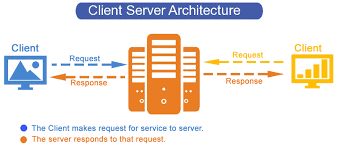
\includegraphics[width=0.8\textwidth]{clientserver}
	\caption{Client server architecture}
	\label{fig:2.10}
\end{figure} 
\paragraph{Peer-to-Peer (P2P)} is a fully distributed architecture which in contrast to client-server has not a centralized service provider. Peers are both clients and servers themselves, P2P promotes sharing of resources and services trough direct exchange between peers. Compared to a centralized client-server architecture a P2P net scales better and typically does not have a single point of failure. 
\begin{figure}[h]
	\centering
	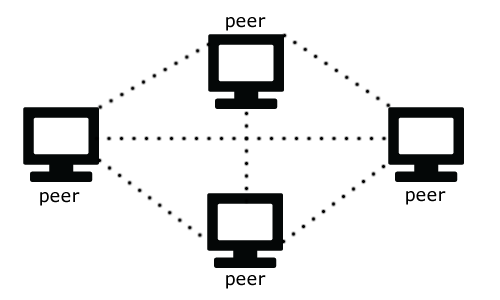
\includegraphics[width=0.8\textwidth]{p2p}
	\caption{P2P architecture}
	\label{fig:2.11}
\end{figure} 
\paragraph{REST style} Representational State Transfer (REST) is a style of architecture based on a set of principles that describe how networked resources are defined and addressed.An application or architecture considered RESTful or REST-style is characterized by:
\begin{itemize}
	\item state and functionality are divided into distributed resources,
	\item every resource is uniquely addressable using a uniform and minimal set of commands (typically using HTTP commands of GET, POST, PUT, or DELETE over the Internet),
	\item the protocol is client/server, stateless, layered, and supports caching.
\end{itemize}



\paragraph{Event based} is an architecture in which components collaborate by exchanging information about occurring events. In particular components in the net can \textit{pubblish} notifications about the events they observe or \textins{subscribe} to events they are interested to be notified about. This architecture can be fully distributed with all the same nodes or can have some semi-centralized nodes which are specialized in computing events or routing messages. Communication is, in this case, purely message based asynchronous and multicast. 
\begin{figure}[h]
	\centering
	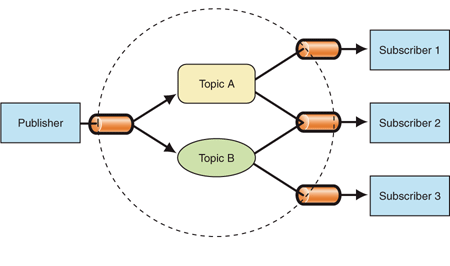
\includegraphics[width=0.8\textwidth]{publishsubscribe}
	\caption{Publish-subscribe architecture}
	\label{fig:2.12}
\end{figure} 

\subsection{Liquid Computation}
\par 





%
% ------------------------------------------------------------------------ %6